% interactcadsample.tex
% v1.03 - April 2017

\documentclass[]{interact}

\usepackage{epstopdf}% To incorporate .eps illustrations using PDFLaTeX, etc.
\usepackage{subfigure}% Support for small, `sub' figures and tables
%\usepackage[nolists,tablesfirst]{endfloat}% To `separate' figures and tables from text if required

\usepackage{natbib}% Citation support using natbib.sty
\bibpunct[, ]{(}{)}{;}{a}{}{,}% Citation support using natbib.sty
\renewcommand\bibfont{\fontsize{10}{12}\selectfont}% Bibliography support using natbib.sty

\theoremstyle{plain}% Theorem-like structures provided by amsthm.sty
\newtheorem{theorem}{Theorem}[section]
\newtheorem{lemma}[theorem]{Lemma}
\newtheorem{corollary}[theorem]{Corollary}
\newtheorem{proposition}[theorem]{Proposition}

\theoremstyle{definition}
\newtheorem{definition}[theorem]{Definition}
\newtheorem{example}[theorem]{Example}

\theoremstyle{remark}
\newtheorem{remark}{Remark}
\newtheorem{notation}{Notation}


% tightlist command for lists without linebreak
\providecommand{\tightlist}{%
  \setlength{\itemsep}{0pt}\setlength{\parskip}{0pt}}



\usepackage{hyperref}
\usepackage[utf8]{inputenc}
\def\tightlist{}
\usepackage{setspace}\doublespacing
\usepackage{graphicx}
\usepackage{nicematrix}
\NiceMatrixOptions{code-for-first-row = \color{red} ,code-for-last-row = \color{red} ,code-for-first-col = \color{blue} ,code-for-last-col = \color{blue}}


\begin{document}


\articletype{Short Technical Note}

\title{Appendix: New and simplified manual controls for projection and
slice tours}


\author{\name{Ursula Laa$^{a}$, Alex Aumann$^{b}$, Dianne
Cook$^{c}$, German Valencia$^{b}$}
\affil{$^{a}$Institute of Statistics, University of Natural Resources
and Life Sciences, Vienna; $^{b}$School of Physics and Astronomy, Monash
University; $^{c}$Department of Econometrics and Business Statistics,
Monash University}
}

\thanks{CONTACT Ursula
Laa. Email: \href{mailto:ursula.laa@boku.ac.at}{\nolinkurl{ursula.laa@boku.ac.at}}, Alex
Aumann. Email: \href{mailto:aaum0002@student.monash.edu}{\nolinkurl{aaum0002@student.monash.edu}}, Dianne
Cook. Email: \href{mailto:dicook@monash.edu}{\nolinkurl{dicook@monash.edu}}, German
Valencia. Email: \href{mailto:german.valencia@monash.edu}{\nolinkurl{german.valencia@monash.edu}}}

\maketitle


\begin{keywords}
data visualisation; grand tour; statistical computing; statistical
graphics; multivariate data; dynamic graphics
\end{keywords}

\hypertarget{refinements-to-enforce-exact-position}{%
\section{Refinements to enforce exact
position}\label{refinements-to-enforce-exact-position}}

The problem with the new simple method (Algorithm 1) is that the precise
values for \(V_m\) cannot be specified because the orthonormalisation
will change them.

\hypertarget{adjustment-method-1}{%
\subsection{Adjustment method 1}\label{adjustment-method-1}}

A small modification to algorithm 1 will maintain the components of
\(V_m\) precisely (Figure \ref{fig:othermethod}). It is as follows:

\begin{enumerate}
\def\labelenumi{\arabic{enumi}.}
\tightlist
\item
  Provide \(A\), and \(m\).
\item
  Change values in row \(m\), giving \(A^*\).
\item
  Store row \(m\) separately, and zero the values of row \(m\) in
  \(A^*\), giving \(A^{*0}\).
\item
  Orthonormalise \(A^{*0}\), using Gram-Schmidt.
\item
  Replace row \(m\) with the original values, giving \(A^{**}\).
\item
  For \(d=2\), adjust the values of \({\boldmath a}^{**}_{.2}\) using
\end{enumerate}

\[a^{**}_{j2}+\frac{a_{m1}a_{m2}}{p-1}, j=1, ..., p, j\neq m.\]

which ensures that

\[\sum_{j=1, j\neq m}^p a^{**}_{j1}a^{**}_{j2} + a_{m1}a_{m2} = 0.\]

If \(d>2\) the process would be sequentially repeated in the same manner
that Gram-Schmidt is applied sequentially to orthormalise the columns of
a matrix. If \(d=1\) no orthonormalisation is needed, and the projection
vector would simply need to be normalized after each adjustment.

\begin{figure}

\includegraphics[width=1\linewidth]{appendix_files/figure-latex/othermethod-1} \caption{Manual controls with algorithm 2. The precise location of the axis is maintained.}\label{fig:othermethod}
\end{figure}

\hypertarget{adjustment-method-2}{%
\subsection{Adjustment method 2}\label{adjustment-method-2}}

For \(d=2\) projections, the projection matrix is the sub-matrix \(A\),
of \(O\) (an orthonormal basis for the p-dimensional space), formed by
its first two columns as illustrated in
Eq.\textasciitilde{}\ref{matrices}. Whereas orthonormality of the basis
for the p-dimensional space is given by
\(e_i\cdot e_j=\delta_{ij},{i,j,=1,\cdots, p}\), orthonormality of the
projection matrix is expressed as
\(\sum_{k=1}^p a_{ki} a_{kj}=\delta_{ij}, ~{i,j=1,2}, ~{k=1,\cdots,p}\).
Movement of the cursor takes the two components \({a_{m1},a_{m2}}\) into
a selected new value \({a^*_{m1},a^*_{m2}}\). Although the motion is
constrained by \(a^{*2}_{m1}+a^{*2}_{m2}\leq 1\), this is not sufficient
to guarantee orthonormality of the new projection matrix. One possible
algorithm to achieve this is

\begin{enumerate}
\item Cursor movement takes ${a_{m1},a_{m2}}\to {a^*_{m1},a^*_{m2}}$, called $V_m$ above.
\item The freedom to change the components $a_{m3}\cdots a_{mp}$ (the columns of $O$ not corresponding to the projection matrix $A$) is used to select a new orthonormal basis as follows:
\begin{enumerate}
\item For row $m$ one chooses $a^*_{m3}=\sqrt{1-a^{*2}_{m1}-a^{*2}_{m1}},~a^*_{m,k>3}=0$
\item For other rows, $a_{i\neq m,j\geq3}$ random selections in the range $(-1,1)$ are made.
\item The Gram-Schmidt algorithm is then used to obtain an orthonormal basis taking $e_m$ as the first vector (which is already normalized), and then proceeding as usual $e_1\to e_1-(e_1\cdot e_m) e_m$, $e_1\to e_1/(e_1\cdot e_1)$, etc, resulting in $A^{**}$.
\end{enumerate}
\item this results in the orthonormal basis $O^*$ and a new projection matrix with $A^{**}_{m1}=a^*_{m1},~A^{**}_{m2}=a^*_{m2}$.
\end{enumerate}

The random completion of \(O\) outside the projection matrix provides an
exploration of dimensions orthogonal to the projection plane. However,
it renders projections in a way that is not continuous and may be
distracting. This can be alleviated by replacing the random completion
with a rule restricting the size of the jumps, for example in step (b)
the values \(a_{i\neq m,j\geq3}\) can be left unchanged before
orthogonalisation.

\begin{align}
O=~~~& \begin{pNiceArray}{ccccc}[first-row,first-col]
\CodeBefore
       \columncolor{red!15}{1,2}
              \rowcolor{blue!15}{4}
     \Body
       & \stackrel{A_1}{\downarrow} & \stackrel{A_2}{\downarrow} &  & &\\
e_1\to & a_{11} & a_{12}  & a_{13} & \cdots & a_{1p} \\
e_2 \to& a_{21}  & a_{22}  & \cdot  &\cdots & a_{2p} \\
\vdots ~~~&\vdots & \vdots  & \vdots & \ddots & \vdots \\ 
 e_m \to& a_{m1}  & a_{m2}  & \cdot  &\cdots & a_{mp} \\   
\vdots ~~~&\vdots & \vdots  & \vdots & \ddots & \vdots \\
e_p \to&a_{p1} & a_{p2} &\cdot &\cdots & a_{pp} 
\end{pNiceArray},\quad (a_{m1},a_{m2})\to (a^*_{m1},a^*_{m2})
\label{matrices}
\end{align}

We could also take a similar approach without completing the basis,
through rotation within the \(d\)-dimensional hyperplane defined by the
new projection. In that case we would again start from \(A^*\) as above,
and then rotate the basis such that the first direction is aligned with
the selected variable \(m\). Applying Gram-Schmid within that basis
definition will not alter the direction for the first vector, thus the
direction of \(m\) remains fixed to what was selected with the cursor.
By adjusting the normalization procedure we can also ensure that the
lenght remains as selcted manually by the user.

\hypertarget{slice-center-guide}{%
\section{Slice center guide}\label{slice-center-guide}}

The slice center, \(c\), from Equation 1 in the main paper, is a point
in the \(p\)-dimensional space. By default, it is placed in the center
of the data (Figure \ref{fig:anchornav} A). Moving this along a variable
axis moves the slice outwards from the center of the data (Figure
\ref{fig:anchornav} B, C). The visual display of the center position is
a form of star plot as suggested useful in \citet{condviz2}, where the
position of the point is marked by a polygon on radial axes indicating
its position relative to the variable minimum to maximum values.

\begin{figure}
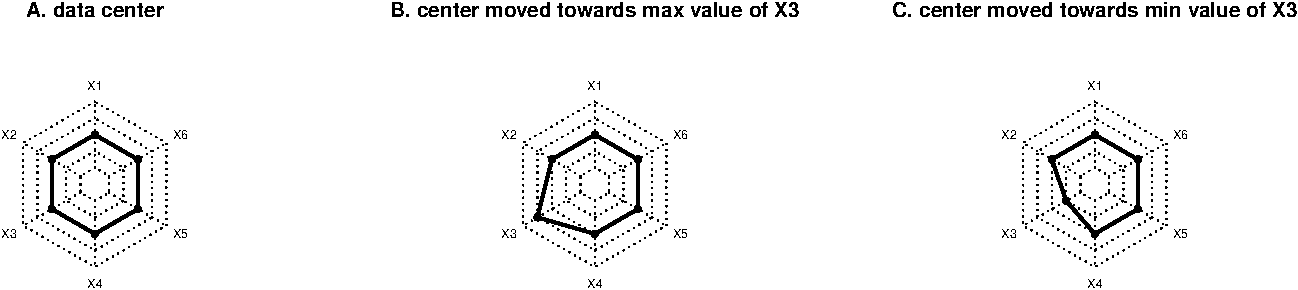
\includegraphics[width=1\linewidth]{appendix_files/figure-latex/anchornav-1} \caption{Visual guide for the slice center. Variable axes are displayed in polar coordinates, where the center corresponds to minimum value and outer end corresponds to maximum value. The position of the center corresponds to the dark polygon. If the center is at the center of the data, this will be displayed as a regular polygon (A), and plots B, C show it's position when moving the center along one axis.}\label{fig:anchornav}
\end{figure}

\hypertarget{software-details}{%
\section{Software details}\label{software-details}}

Here we describe the functions implemented in the Mathematica package
\texttt{mmtour.wl}. The main function and its arguments are given below:

\texttt{SliceDynamic{[}data,\ projmat,\ height,\ heightRange,\ legendQ(=1),\ flagQ(=1),\ colorFunc(=ColorData{[}97{]}){]}}

\begin{itemize}
\tightlist
\item
  \texttt{data}: A data matrix, potentially with grouping that has a
  label (string) and a flag (numerical) in the last two columns.
\item
  \texttt{projmat}: The initial projection matrix. It is possible to
  start with a random projection with the input ``random'' (including
  the quotes) in this entry field.
\item
  \texttt{height}: The initial height of the slice.
\item
  \texttt{heightRange}: The range of slice heights to be explored.
\item
  \texttt{legendQ}: A flag signaling whether the data matrix includes a
  column with group labels (1) or not (0).
\item
  \texttt{flagQ}: A flag signaling whether the data matrix includes a
  numerical flag for the groups.
\item
  \texttt{colorFunc}: specifies the color mapping for the different
  groups.
\end{itemize}

The first four arguments are required. As possible starting values we
suggest using a random input projection, and selecting slice height
parameters using the estimate given in Section 2.4.2 of the paper.

The function renders a manual tour with controls that allow the user to
navigate through different projections. For a given projection, a slider
permits the user to change the slice width within its range and a
separate box switches the view to a projection. The user can also change
the center point of slices; the size of the points rendered and the
scale of the plot through sliders. An additional box displays the
coordinates of the projection matrix explicitly.

This function can be used for ungrouped data by setting legendQ and
flagQ to 0. To remove a group from the visual display, the user can
choose specific colors for the entry colorFunc. For example,
\{Red,White,Green\} would display groups 1 (red) and 3 (green) while
making 2 invisible.

The package includes the additional functions not used in the example
application: \texttt{ProjectionPlot}, \texttt{Projected2DSliderPlot},
and \texttt{VisualiseSliceDyanmic}.

\texttt{ProjectionPlot} is very similar to \texttt{SliceDynamic}, except
it only displays projections. Using it instead of \texttt{SliceDynamic}
simplifies the display and is more efficient. The interface is slightly
different, the data file should not contain labels for groups, if these
are desired they are passed through the optional argument legendNames as
\{``group 1'', ``group 2'',\ldots\}, for example. The function and its
arguments are given below:

\texttt{ProjectionPlot{[}data,\ projmat,\ legendNames(=\{\}),\ colorFunc(=ColorData{[}97{]}){]}}

\begin{itemize}
\tightlist
\item
  \texttt{data}: A data matrix with one or more groups labeled by a flag
  (numerical, last column).
\item
  \texttt{projmat}: The initial projection matrix. It is possible to
  start with a random projection with the input ``random'' (including
  the quotes) in this entry field.
\item
  \texttt{legendNames}: an optional list of labels for the groups.
\item
  \texttt{colorFunc}: specifies the color mapping for the different
  groups.
\end{itemize}

\texttt{ProjectedLocatorPlot} displays the interactive controls slightly
differently. Several locator panes are displayed above the display of
the projected data and each one corresponds to a row in the projection
matrix. The updating behavior of the projection is the same as in
\texttt{ProjectionPlot}. The function and its arguments are given below:

\texttt{ProjectedLocatorPlot{[}data,\ projmat,\ legendNames(=\{\}),\ colorFunc(=ColorData{[}97{]}){]}}

\begin{itemize}
\tightlist
\item
  \texttt{data}: A data matrix with one or more groups labeled by a flag
  (numerical, last column).
\item
  \texttt{projmat}: The initial projection matrix. It is possible to
  start with a random projection with the input ``random'' (including
  the quotes) in this entry field.
\item
  \texttt{legendNames}: an optional list of labels for the groups.
\item
  \texttt{colorFunc}: specifies the color mapping for the different
  groups.
\end{itemize}

Finally \texttt{VisualiseSliceDynamic} allows to discern which points
exist inside the slice and outside it. This function differs from
\texttt{SliceDynamic} in that it looks at only one data set but displays
both the points inside and outside the slice. The display panel allows
the user to specify the size of both sets of points (inside and outside)
along with the slice height, center point and zoom level. The function
and its arguments are given below:

\texttt{VisualiseSliceDynamic{[}data,\ projmat,\ height,\ heightRange{]}}

\begin{itemize}
\tightlist
\item
  \texttt{data}: A data matrix containing only one group. In this case
  the data matrix should not contain column labels.
\item
  \texttt{projmat}: The initial projection matrix. It is possible to
  start with a random projection with the input ``random'' (including
  the quotes) in this entry field.
\item
  \texttt{height}: The initial height of the slice.
\item
  \texttt{heightRange}: The range of slice heights to be explored.
\end{itemize}

The points inside the slice are shown in black whereas those outside the
slice are shown in light blue, with labels indicating this.

\bibliographystyle{tfcad}
\bibliography{biblio.bib}





\end{document}
